\subsubsection{Percentuale di requisiti soddisfatti}

    \begin{figure}[H]
        \centering
        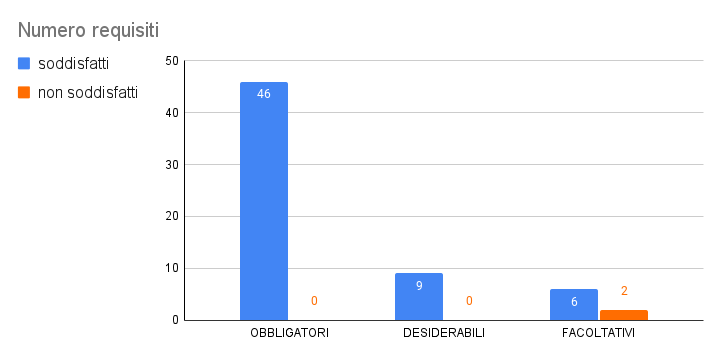
\includegraphics[width=15 cm]{source/sections/images/num-requisiti.png}
        \caption{Grafico dei requisiti}
    \end{figure}

    \begin{figure}[H]
        \centering
        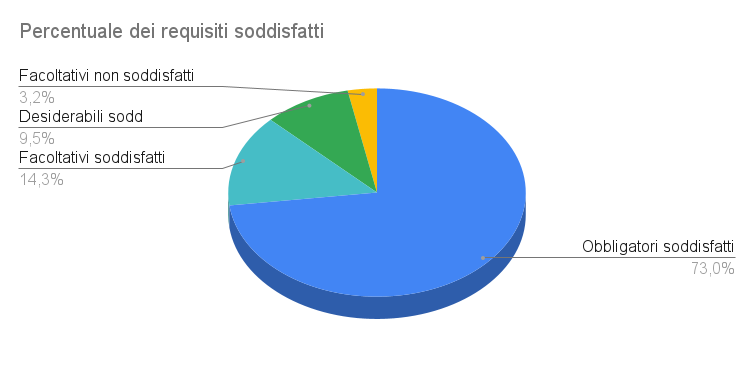
\includegraphics[width=15 cm]{source/sections/images/percentuale-requisiti.png}
        \caption{percentuale dei requisiti soddisfatti}
    \end{figure}

\subsubsection{Metriche di pianificazione}
    Le metriche di pianificazione che mostrano il rispettare dei costi e dei tempi sono stati calcolati in questa versione del documento in 4 gruppi denotati dalle seguenti sigle:
    \begin{itemize}
        \item \textbf{An}: Periodo di analisi, ovvero dal 26-11-2020 al 10-01-2021
        \item \textbf{CC}: periodo di consolidamento dei requisiti, ovvero dal 12-01-2021 al 18-01-2021
        \item \textbf{PA}: Progettazione architetturale, ovvero dal 19-01-2021 al 01-03-2021, che rappresenta la data progettata per la consegna
        \item \textbf{PAS}: Progettazione architetturale con consegna "a sportello", ovvero dal 02-03-2021 al 10-03-2021, che rappresenta la data spostata con consegna il 10 marzo
        \item \textbf{PDC}:Progettazione di dettaglio e codifica, dal 11-03-2021 al 20-04-2021
    \end{itemize}
    
    
    \begin{longtabu} to \textwidth {| X[0.1,c m] | X[0.1,c m]| X[0.1,c m]| X[0.1,c m]| X[0.1,c m]| X[0.1,c m] |}
        \hline
        \rowcolor{header}
        \textbf{Fase} &
        \textbf{EV} &
        \textbf{PV} &
        \textbf{AC} &
        \textbf{SV} &
        \textbf{CV} \\
        \hline
        An & - & - & - & - & -  \\ 
        \hline
        CR & 734 & 734 & 650 & 0 & 84 \\
        \hline
        PA & 2588 & 3624 & 3439 & -1035 & -841\\
        \hline
        PAS & 1035 & 0 & 966 & 0 & 69 \\
        \hline
        PDC & 5935 & 5935 & 5935 & 0 & 69 \\
        \hline 
        \end{longtabu}


        \begin{figure}[H]
            \centering
            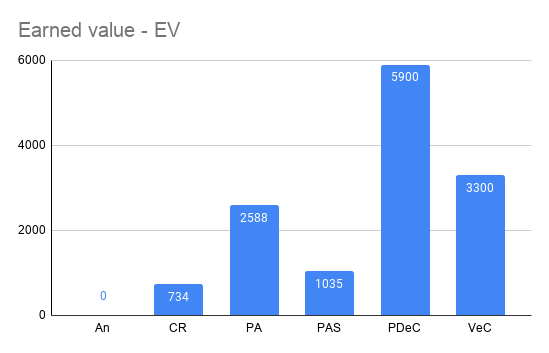
\includegraphics[width=11 cm]{source/sections/images/Earned_value.png}
            \caption{Grafico dei valori dell'Earned value}
        \end{figure}

        \begin{figure}[H]
            \centering
            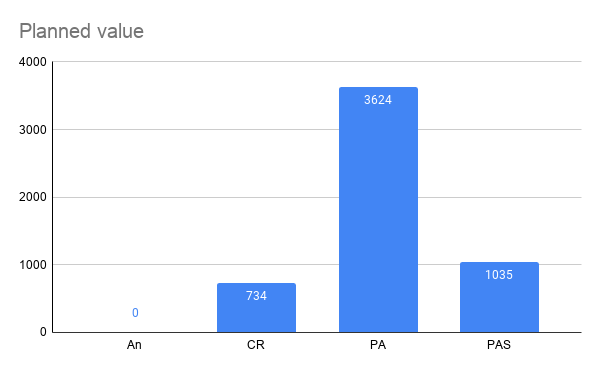
\includegraphics[width=11 cm]{source/sections/images/planned_value.png}
            \caption{Grafico dei valori del Planned value}
        \end{figure}


        \begin{figure}[H]
            \centering
            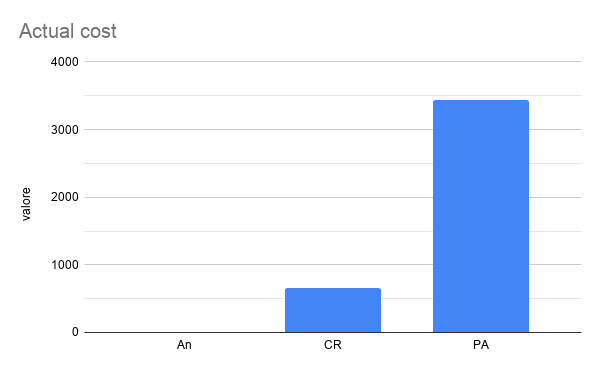
\includegraphics[width=11 cm]{source/sections/images/actual_cost.png}
            \caption{Grafico dei valori dell'Actual cost}
        \end{figure}


        \begin{figure}[H]
            \centering
            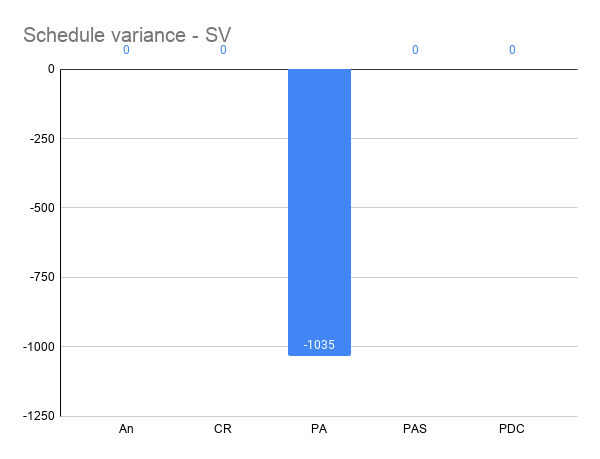
\includegraphics[width=11 cm]{source/sections/images/schedule_variance.png}
            \caption{Grafico dei valori dello Schedule variance}
        \end{figure}


        \begin{figure}[H]
            \centering
            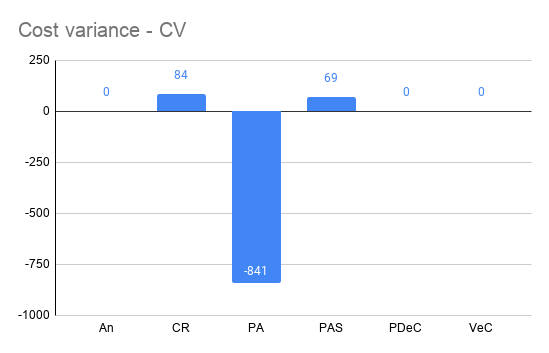
\includegraphics[width=11 cm]{source/sections/images/cost_variance.png}
            \caption{Grafico dei valori del Cost variance}
        \end{figure}